\documentclass[12pt,oneside]{article}

%%%%%%%%%%%%%%%%%%%%%%%%%%%%
%%   Zusaetzliche Pakete  %%
%%%%%%%%%%%%%%%%%%%%%%%%%%%%
\usepackage{enumerate}  
\usepackage{fancyhdr}
\usepackage{a4wide}
\usepackage{graphicx}
\usepackage{palatino}
\usepackage{multirow}
\usepackage{booktabs}
\usepackage{titlesec}
\usepackage{acronym}% http://ctan.org/pkg/acronym
\usepackage{enumitem}% http://ctan.org/pkg/enumitem
\usepackage{pythonhighlight}
\usepackage{listings}
\usepackage{minted}
\usepackage{xcolor}
\usepackage{pgf} 
\usepackage{pythonhighlight}
%folgende Zeile auskommentieren für englische Arbeiten
\usepackage[ngerman]{babel}
%folgende Zeile auskommentieren für deutsche Arbeiten
%\usepackage[ngerman, english]{babel}

\usepackage[T1]{fontenc}
\usepackage[utf8]{inputenc}
\usepackage[bookmarks]{hyperref}
\usepackage[justification=centering]{caption}
\usepackage[style=authoryear,natbib=true,backend=biber,maxbibnames=20]{biblatex}
\usepackage{csquotes}
\bibliography{literatur}

\setlength{\parindent}{0em} 
\setlist[itemize]{noitemsep, topsep=0pt}
\setlist[enumerate]{noitemsep, topsep=0pt}

\newcommand{\subsubsubsection}[1]{\paragraph{#1}\mbox{}\\}
\setcounter{secnumdepth}{4}
\setcounter{tocdepth}{4}
%%%%%%%%%%%%%%%%%%%%%%%%%%%%%%
%% Definition der Kopfzeile %%
%%%%%%%%%%%%%%%%%%%%%%%%%%%%%%

\pagestyle{fancy}
\fancyhf{}
\cfoot{\thepage}
\setlength{\headheight}{16pt}

%%%%%%%%%%%%%%%%%%%%%%%%%%%%%%%%%%%%%%%%%%%%%%%%%%%%%
%%  Deckblatt (Platzhalter)  %%
%%%%%%%%%%%%%%%%%%%%%%%%%%%%%%%%%%%%%%%%%%%%%%%%%%%%%
\thispagestyle{empty}
%Platzhalter für späteres Deckblatt
\hspace{-2cm}
\includegraphics{pabu5097_3677_cover.pdf}
\newpage

%%%%%%%%%%%%%%%%%%%%%%%%%%%%
%%  Beginn des Dokuments  %%
%%%%%%%%%%%%%%%%%%%%%%%%%%%%

\begin{document}

\lhead{}
\pagenumbering{Roman} 
    \setcounter{page}{1}

\tableofcontents
\clearpage
%Gendererklärung
\addcontentsline{toc}{section}{Gendererklärung}
\lhead{Gendererklärung}
\section*{Gendererklärung}
Aus Gründen der besseren Lesbarkeit wird in dieser Bachelorarbeit auf die gleichzeitige Verwendung der Sprachformen männlich, weiblich und divers (m/w/d) verzichtet. Sämtliche Formulierungen gelten gleichermaßen für alle Geschlechter.
%%%%%%%%%%%%%%%%%%%%%%%%%%%%
%%  Kurzzusammenfassung   %%
%%%%%%%%%%%%%%%%%%%%%%%%%%%%
\lhead{Zusammenfassung}
%\section*{Zusammenfassung}
\addcontentsline{toc}{section}{Zusammenfassung}
\newpage
\newpage
\begin{otherlanguage}{ngerman}
\section*{Zusammenfassung}

In dieser Arbeit soll das Thema der forensischen Analyse von schädlicher Software behandelt werden. Explizit ist damit gemeint, dass eine Umgebung für diese Untersuchung in wenigen Sekunden geschaffen werden kann, welche den nötigen Sicherheitsstandards entspricht und so eine sichere Beobachtung des Malwareverhaltens gewährleisten kann. Diese Umgebung soll unabhängig vom Anbieter mit den selben Werkzeugen erstellt werden. So kann im Notfall schnell gehandelt werden, um festzustellen, welche Systemkomponenten von einem Angriff gefährdet sind.
\newline Somit ist diese Arbeit im Bereich der IT-Security und Datensicherheit anzusiedeln. Dies sind in der heutigen Zeit wichtige Themenbereiche um den Schutz aller Daten bieten zu können.
\end{otherlanguage}

\lhead{Abstract}
\section*{Abstract}
\addcontentsline{toc}{section}{Abstract}



\newpage
\lhead{Abbildungsverzeichnis} 
\addcontentsline{toc}{section}{Abbildungsverzeichnis} 
\listoffigures

\newpage
\lhead{Tabellenverzeichnis}
\addcontentsline{toc}{section}{Tabellenverzeichnis} 
\listoftables
\newpage

\setlength{\parskip}{0.5em} 


%%%%%%%%%%%%%%%%%%%%%%%%%%%%%%%%%%
%%  Definition der Abkürzungen  %%
%%%%%%%%%%%%%%%%%%%%%%%%%%%%%%%%%%
\lhead{Abkürzungsverzeichnis} 

\addcontentsline{toc}{section}{Abkürzungsverzeichnis}  
\begin{otherlanguage}{ngerman}
\section*{Abkürzungsverzeichnis} 
\begin{acronym}
 \acro{VM}{Virtuelle Maschine}
 \acro{SSH}{Secure Shell}
 \acro{DNS}{Domain Name System}
 \acro{IaaS}{Infrastructure as a Service}
 \acro{PaaS}{Platform as a Service}
 \acro{SaaS}{Software as a Service}
 \acro{OS-Image}{Operating System-Image}
 \acro{SSD}{Solid State Drive}
\end{acronym}
\end{otherlanguage}

\newpage
%%%%%%%%%%%%%%%%%%%%%%%%%%%%
%%  Glossar  %%
%%%%%%%%%%%%%%%%%%%%%%%%%%%%
\lhead{Glossar} 
%\section*{Glossar} 
\addcontentsline{toc}{section}{Glossar}  
\newpage
\begin{otherlanguage}{ngerman}
\section*{Glossar}
\begin{acronym}
 \acro{App}{- ist eine Anwendung}
 \acro{Cloud}{- ist in der IT die Abkürzung für Cloud Computing und wird auch als Rechnerwolke oder Datenwolke bezeichnet}
 \acro{Cloud Server}{- ist ein virtueller Server. Dieser bezieht seine Hardwarekomponenten von externen Dienstleistern und wird über das Internet angeboten.}
 \acro{Firewall}{- ist ein Sicherungssystem um Netzwerke und Computer vor unerewünschten Zugriffen zu schützen}
 \acro{Open-Source-Software}{- ist Software deren Quellcode der Öffentlichkeit zugänglich ist. Die Benutzung des Codes steht dem Benutzer selbst offen.}
 \acro{OS-Images}{- ist eine komprimierte Sammlung von Referenzdateien und Ordnern, die zum Installieren und Konfigurieren eines neuen Betriebssystems auf einem Computer verwendet werden}
 \acro{Workflow}{- die Abwicklung arbeitsteiliger Vorgänge}
 \acro{Cloud Provider}{- Anbieter für Cloud Computing}
\end{acronym}
\end{otherlanguage}
%%%%%%%%%%%%%%%%%%%%%%%%%%%%
%%  Einstellungen  %%
%%%%%%%%%%%%%%%%%%%%%%%%%%%%
\clearpage
\pagenumbering{arabic}  
    \setcounter{page}{1}
\lhead{\nouppercase{\leftmark}}

%%%%%%%%%%%%%%%%%%%%%%%%%%%%
%%  Hauptteil  %%
%%%%%%%%%%%%%%%%%%%%%%%%%%%%
\lhead{Einleitung}
%Einleitung
\section{Einleitung} 

\subsection{Thema der Arbeit und Motivation}
In dieser Arbeit geht es um die Nutzung virtueller Umgebungen für die Analyse von schädlicher Software in einem automatisierten Verfahren. Dabei entstehen im Bereich der virtuellen Umgebung besonders komplexe Probleme, wie die Auswahl der Tools, des Betriebssystems oder des Cloud-Anbieters. Außerdem wird die Frage aufgeworfen, wie eine virtuelle Umgebung automatisiert und flexibel erstellt werden kann. Dabei ist die Unabhängigkeit vom Anbieter besonders wichtig, da das Malware-Analyse-Labor so flexibel sein soll, dass es bei vielen verschiedenen Anbietern mit wenig Aufwand konfiguriert und verwendet werden kann. 
\newline 
Wenn diese Umgebung erstellt wurde, ist es wichtig, dass diese sicher ist, denn Malware sollte nicht auf Rechnern mit sensiblen Daten Zugriff haben. Das heißt, dass die Art, wie die virtuelle Umgebung nach außen abgesichert ist, eine grundlegende Rolle für die Funktion dieser spielt. Allgemein soll durch diese Arbeit die persönliche IT-Sicherheit vereinfacht und verbessert werden. Daher ist die Absicherung einer der wichtigsten Punkte. Zu diesen wichtigen Punkten zählt unter anderem auch die Auswahl der Tools. Diese legt fest, wie die Umgebung später genutzt wird.
\newline
Weitere Punkte, die außerdem aufgegriffen werden, sind die Konfiguration der Kommunikationsmöglichkeiten, die der Analyse-Umgebung zur Verfügung stehen. Um hier feste Aussagen treffen zu können, muss die allgemeine Funktionsweise verschiedener Malwarearten durchblickt werden.
\subsubsection{Relevanz}
Malware-Analyse gibt Auskunft über das Verhalten von der untersuchten Schadsoftware. Die Informationen, die dabei gewonnen werden, können für die Sicherheitsmaßnahmen des Zielsystems wichtige Aufschlüsse darüber geben, wie das Eindringen dieser Malware-Art in das System in Zukunft unterbunden werden kann.
\newline Außerdem kann die Funktionalität der Malware unterbunden werden, wenn bekannt ist, mit welchen Ressourcen die Malware arbeiten muss, um zu funktionieren. Alles in Allem bietet Malware-Analyse eine große Bereicherung für die IT-Sicherheit. Das Problem dabei ist oft, dass die notwendige Umgebung für die Analyse von Malware nicht überall vorhanden ist. Es besteht die Möglichkeit des Mietens solcher Umgebungen bei externen Firmen, was aber teilweise sehr kostspielig ist. Die Grundlage für eine Alternative dazu soll in dieser Arbeit geschaffen werden.
\subsection{Forschungsstand}
Malware-Analyse und die Erstellung dieser ist ein Thema mit hohem Stellenwert in der IT. Der Forschungsstand zu einzelnen Malwarearten, sowie zu der Malware-Analyse, ist ein dementsprechend gut erforschtes Themengebiet mit vielen wissenschaftlichen Publikationen. Auch \dq Terraform \dq{} als Provisioning-Tool für Cloud-Umgebungen ist nicht unbekannt. Es finden sich daher auch hierzu wissenschaftliche Artikel und Publikationen, die den Umgang und die Möglichkeiten des Tools betrachten. 
\newline
In dieser Arbeit sollen diese beiden Parts zusammengefügt werden, denn bei der Recherche ist auffällig geworden, dass die beiden Themen nur separat voneinander untersucht wurden. Daher sollen sie hier verbunden werden, um die Möglichkeiten aufzuzeigen, die Terraform in der Welt der Malware-Analyse bietet. Dazu liegen bis zum jetzigen Zeitpunkt wenig bis keine Arbeiten und Publikationen vor.
\subsection{Aufbau der Arbeit}
Zunächst wird im zweiten Kapitel eine theoretische Grundlage geschaffen. Diese ist untergliedert in Grundlagen zu \dq Terraform\dq, zu Cloud Computing, zu virtuellen Maschinen und zu Malware, sowie ihrer Analyse. 
\newline Anschließend befasst sich Kapitel drei mit dem praktischen Teil dieser Arbeit. Dafür wird das Vorgehen mit den einzelnen Werkzeugen, um das Ziel zu erreichen, beschrieben. Hierbei zeigt der Teil Terraform \ref{Praktisches Terraform} auf, wie die Konfigurationsdateien aussehen. Im Anschluss dazu geht es um die virtuelle Umgebung, die aus den entsprechenden Konfigurationsdateien hervorgeht. Die Tools, die hier installiert sind, werden im nächsten Punkt genauer erläutert. Hier wird einerseits auf die einzelnen Tools eingegangen, andererseits ist hier auch der Zweck dieser Tools erklärt.
\newline
Im vierten Kapitel werden die Ergebnisse dargestellt. Dazu wird die tatsächliche Vorgehensweise dargelegt und die Verwendung, der in Kapitel drei genannten Methoden, aufgezeigt. Außerdem werden hier die Ergebnisse und deren Aussagekraft über die Forschung eingeordnet. 
\newline
Das fünfte Kapitel ist die Diskussion, in welcher die Ergebnisse genauer interpretiert und bewertet werden. Auch mögliche Verbesserungsvorschläge sind hier aufzugreifen.
\newline
Als Abschluss dieser Arbeit steht das Fazit im sechsten Kapitel. Dort werden die wichtigsten Erkenntnisse, aus der Forschung, im Rahmen der Arbeit dargelegt. Anschließend folgt das Literaturverzeichnis, sowie der Anhang.
\subsection{Ziel der Arbeit}
Das konkrete Ziel dieser Arbeit ist es, die Möglichkeit zu bieten, mithilfe bestimmter Tools eine virtuelle Umgebung für die Analyse von Malware zu erstellen. Der Fokus liegt darauf, dass die Flexibilität dieser Umgebung geboten wird. Außerdem sollen für jede Analysetechnik Tools zur Verfügung stehen. Ein weiterer Faktor, der beachtet wird, ist, dass die Kosten für diese Umgebung sehr günstig im Vergleich zu den kommerziellen Lösungen sind. So ist das Ziel, jedem, der Malware analysieren möchte oder muss, eine kostengünstige, erste Grundlage bieten zu können, um die Analyse durchführen zu können.


\lhead{Theoretische Grundlagen}
%Theoretische Grundlagen
\subsection{Terraform}
\begin{otherlanguage}{ngerman}
\subsubsection{Funktionsweise}
\textit{Terraform} ist eine \textit{Open-Source-Software}, welche die Vorbereitung von \textit{Cloud Servern} einfacher macht. Sie wurde von HashiCorp dazu entwickelt, Infrastrukturen vorzubereiten und zu verwalten.\footcite{introform} Mit Infrastrukturen sind hier \textit{virtuelle Maschinen} verschiedenster Anbieter gemeint.\footnote{\cite{Terraform}} Terraform hat lizenzierte Partner für die seine Dienste anwendbar sind.\footcite{TerraProviders} Durch die hohe Konnektivität dieser Software sind die Einsatzorte sehr vielseitig. Das macht die Software in der Entwicklung und im Betrieb von Unternehmen sehr attraktiv. 
\newline
\newline
Terraform ist ein Infrastructure-as-Code-Tool und wird für die Bereitstellung von physischen als auch virtuellen Servern verwendet. Das Tool arbeitet mit Konfigurationsdateien, die in der HashiCorp Configuration Language(HCL) geschrieben werden. Die genannten Dateien sind von Menschen lesbar und gewährleisten dadurch die geringe Komplexität der Sprache. Zudem ist HCL eine deklarative Sprache. Das heißt, dass der Nutzer den Wunschaufbau des Servers in der Terraform-Datei beschreibt. Die einzelnen Schritte um den gewünschten Serverzustand zu erreichen werden von Terraform übernommen. 
\newline
Die Prozesse in die die Arbeit mit Terraform unterschieden werden kann, sind in drei Schritte aufgeteilt. Der erste Schritt ist \tt write \rm. In dieser Phase wird der Code definiert. Dafür werden die benötigten Ressourcen für die jeweiligen Provider definiert. Dafür Terraform-Konfigurations-Dateien mit der Endung \tt .tf \rm verwendet. Aus diesen Dateien entnimmt Terraform beispielsweise welcher Cloud-Anbieter verwendet wird. Als Beispiel für einen Anbieter mit dem Terraform funktioniert können die Microsoft Azure-Dienste genannt werden. Zu den Providern findet sich auf der Seite von Terraform eine jeweilige Dokumentation darüber, wie die Ressourcen einzubinden sind. Der Code der Konfigurations-Dateien entscheidet darüber, wie der Server konfiguriert wird, wenn dass script ausgeführt wird. 
\newline
Wenn der Code verfasst wurde folgt der nächste Schritt im Arbeitsablauf von Terraform. Dieser ist die Planung der vorgenommenen Aktionen. Wird \tt terraform apply \rm in der Kommandozeile eingegeben so wird dieser Plan erstellt. Dieser wird im Anschluss daran ausgegeben. Um Fortzufahren muss der Plan, indem jeder Schritt aufgelistet ist, den Terraform durchführen wird, bestätigt werden. Diese einzelnen Schritte können Änderungen, Löschungen oder das Hinzufügen von Dateien sein.
\begin{figure}
    \centering
    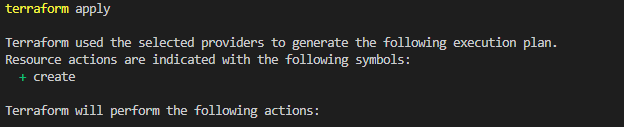
\includegraphics{LaTeX/graphic/terraformapply.png}
    \caption{Terraform - Planungsphase}
\end{figure}
%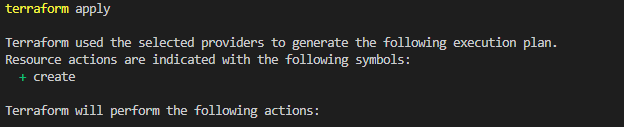
\includegraphics[]{LaTeX/graphic/terraformapply.png}

\newpage 
Die Dritte und letzte Phase im Terraform-Workflow ist \tt apply \rm. Sie beginnt mit der Bestätigung des Plans. Ab diesem Zeitpunkt beginnt Terraform mit der Bereitstellung des Servers. Welche Systemkomponenten und Sicherheitseinstellungen dieser hat ist von den Konfigurationsdateien abhängig. 
\newpage
\subsubsection{Vorteile}
-schnell
\newline
-variabel
\newline
-nicht allzu komplex
\end{otherlanguage}
\begin{otherlanguage}{ngerman}
\subsection{Cloud Computing}
Cloud Computing (\it deutsch Rechnerwolke oder Datenwolke \rm) ist das Bereitstellen von einzelnen Anwendungen bis hin zu Rechenzentren. Die Ressourcen hierfür werden aus der \it Cloud \rm genommen, welche auch als \it Internet \rm bekannt ist. Durch flexible Einstellungsoptionen ist es durch Cloud Computing möglich IT-Systeme bedarfsspezifisch und flexibel anzubieten. Dabei ist auch zu beachten, dass Cloud Computing viele Vorteile mit sich bringt. Darunter fallen beispielsweise die Kosten und die Skalierbarkeit virtueller Systeme. 
\newline 
Cloud Computing wird in drei Arten aufgeteilt: Public (öffentlich), Privat (privat) und Hybrid (Mischung aus öffentlich und privat). Bei der öffentlichen Form besitzt ein Dienstleister die benötigten Ressourcen, welchen man \it Cloud Provider \rm nennt. Dabei werden die, den Kosten entsprechenden Komponenten, dem Kunden über das Internet zur Verfügung gestellt. Hier spielen die Kosten, als Vorteil, eine große Rolle, da die Hardware nicht selbst angeschafft werden muss. Zudem sind Hardware-Wartungen nicht nötig, da diese vom \it Cloud Provider \rm übernommen werden. Durch die Vielzahl an Komponenten, die große Anbieter bieten können, steigt die Skalierbarkeit sehr stark. Die Servermenge in den Rechenzentren der Provider ist außerdem ausschlaggebend dafür, dass das Risiko eines Ausfalls minimiert wird. 
\newline
Die private Form des Cloud Computings unterscheidet sich von der öffentlichen Form. Besonders im Aspekt des Zugriffs auf die Hardware treten Unterschiede auf. Während bei der öffentlichen Form die selbe Hardware von verschiedenen Kunden genutzt wird, wird die Hardware bei privaten Cloud Computing-Lösungen nur einem Kunden zugewiesen. Diese kann hierbei im Besitz des Kunden sein und sich in seiner Organisation befinden. Auch kann sich die Hardware in Räumen von Drittanbietern befinden. Dabei ist sie dennoch nur für einen Käufer der Systemkomponenten bestimmt. So können Unternehmen ihre Netzwerkrichtlinien souverän bestimmen. Zudem gewährleistet die private Nutzung von Hardware mehr Sicherheit. 
\newline
In der hybriden Form sind die beiden vorangegangenen Modelle vereint. Ziel dabei ist es die Vorteile beider Formen in einer Form zu verschmelzen. Beispielsweise kann die große Flexibilität von öffentlichen Clouds benutzt werden. Währendessen stellt die private Cloud, durch ihre höhere Sicherheit, eine Zone für Komponenten des Netzwerkes da. Aus der Zusammenführung der beiden Modelle ergibt sich eine Form, die die Vorteile vereint. Die Netzwerkkontrolle ist geboten, die Kosteneffizienz ist hoch und es wird ein hohes Maß an Flexibilität und Skalierbarkeit geboten. 

\subsubsection{Die Arten von Cloud-Diensten}
\bf Infrastructure as a Service (IaaS)\rm oder zu deutsch: \it Infrastruktur als Dienstleistung \rm stellt die notwendigen Systemkomponenten bereit. Dazu zählen beispielsweise der Arbeitsspeicher, die Festplatte oder der Prozessor. Diese Komponenten können von Drittanbietern oder von der Organisation selbst bereitgestellt werden. In dieser Kategorie sind \it Amazon Web Services\rm,  \it Microsoft Azure\rm oder auch die  \it Hetzner Cloud \rm einzuordnen. Diese bieten das digitale bereitstellen von Cloud-Umgebungen an. Diese Umgebungen können an die Anforderungen angepasst und flexibel erweitert werden. So zahlt der Nutzer nur für das, was er benutzt. Zudem muss er so keine Hardware für seine Cloud-Umgebung selber bereitstellen. 
\newline 
\bf Platform as a service (PaaS) \rm  oder zu deutsch: \it Plattform als Dienstleistung \rm stellt die Platform für Entwicklungen und Anwendungen bereit. Diese wird von der folgenden Dienstleistung \it Software as a service (SaaS) \rm benötigt. Nutzer von PaaS sind zum Beispiel Anwendungsentwickler die in großen Teams zusammen an einem Projekt arbeiten. Als Vertreter von \it PaaS \rm -Produkten kann \it Google App Engine \rm genannt werden. Hier stehen für den Nutzer verschiedene Entwicklungsprachen zur Verfügung. Der Vorteil ist, dass viele Aufgaben die Entwickler übernehmen müssten um eine skalierbare Software zu schreiben, von Google übernommen werden. Somit werden die Arbeitszeit und Kosten verringert.
\newline 
\bf Software as a service (SaaS) \rm befasst sich mit der Software von Systemen. Eine Software ist eine Anwendung für einen Computer. Der Inhalt der Software legt fest was bei seiner Ausführung auf dem Computer passiert. Der ausführende Teil wird von der Hardware übernommen. Bei Software aus dem Modell \it SaaS \rm werden Anwendungen, die cloudbasiert arbeiten können angeboten. Diese sind in der Regel skalierbar, sodass sie auf Wünsche einzelner Organisationen eingehen können. Darunter fällt beispielsweise das Tool des Softwarekonzerns SAP \it Enterprise Resource Planning \rm. Dieses Tool ist für Unternehmen gedacht und kann Prozesse im Zusammenhang betrachten und beispielsweise analysieren. Hier wird klar, dass die Skalierbarkeit von \it SaaS \rm große Vorteile bringt. So kann Software individuell auf Unternehmen angepasst werden, um den einzelnen Anforderungen gerecht zu werden. 
\end{otherlanguage}

\begin{otherlanguage}{ngerman}
\subsection{Virtuelle Maschinen}
\subsubsection{Was ist eine virtuelle Maschine?}
Virtuelle Maschinen bilden mit Infrastructure as a Service (IaaS) eines der drei Servicemodelle des Cloud Computings. Sie beruhen auf der Idee Hardware, Rechenleistung, Speicherplatz und Netzwerkressourcen aus der Cloud bereitzustellen. So hat der Benutzer von virtuellen Maschinen das gleiche Erlebnis wie er es auch bei physischen Geräten hat. 
\newline 


\subsubsection{Erstellen einer virtuellen Maschine}
Eine virtuelle Maschine kann in der Regel bei einem \it Cloud Provider \rm erstellt werden. Hierfür kann die grafische Umgebung der jeweiligen Provider genutzt werden. Bevor jedoch eine VM erstellt wird muss darüber nachgedacht werden zu welchem Zweck die VM ist. Daraus ergeben sich wichtige Konfigurationsmerkmale wie das Betriebssystem oder die Sicherheitskonfigurationen. 
\newline
-Terraform

\subsubsection{Absicherung einer virtuellen Maschine}
Die Sicherung der virtuellen Maschine kann je nach Einsatzgebiet eine große Bedeutung haben. Um Sicherheitskonfigurationen einzubinden kann die Firewall bearbeitet werden. Auch dafür bietet Terraform eine Möglichkeit. 
\newline 
-Terraform
\end{otherlanguage}
\begin{otherlanguage}{ngerman}
\subsection{Malware}
\subsubsection{Was ist Malware und wie funktioniert sie?}

Laut Defintion ist Malware eine "bösartige Software"
(auf Englisch "malicious software").
\newline Allgemein dient der Begriff Malware als Klassifizierung von Dateien oder Software, die Schäden verursachen, sobald sie sich im System des Benutzers befinden. 
\newline Die häufigsten Arten sind:
\begin{enumerate}
    \item Viren
    \item Trojaner
    \item Würmer
    \item Spyware/Adware
    \item Scareware
    \item Ransomware
    \item Root kit und Backdoors
\end{enumerate}
Dabei können sowohl persönliche Schäden als auch Sachschäden entstehen.

Um einen solchen Malware Angriff zu tätigen, benötigt man einen Schadcode. 
Mithilfe dessen verschaffen sich Angreifer Zugriff auf das System des Opfers und klauen Passwörter oder andere sensible Daten.
Um den Datendiebstahl durchzuführen, muss ein Angreifer dafür sorgen, dass der Schadcode auf dem Zielsystem ausgeführt wird. 
Damit das klappt, betten diese den schädlichen Code in eine Datei ein, die das Opfer öffnen soll.
Nach der Durchführung erfüllt der Schadcode seinen Zweck und installiert zum Beispiel eine Backdoor oder startet einen Key-Logger. Key Logger können unter anderem die Eingabe von Passwörtern protokollieren.

\subsubsection{Arten von Malware}
Neue Schadprogramm Varianten entstehen, wenn die Funktionsweise der neuen Malware grundlegend von bereits vorhandenen Schadprogrammen abweicht. Wichtig ist hierbei, dass der Hashwert einzigartig ist, aber ein neuer Hashwert nicht mit einer neuen Malware gleichzusetzen ist. Das Ergebnis einer Hashfunktion unterscheidet sich bereits bei geringfügigen Veränderungen im Programmcode. Das heißt, dass ein neuer Hashwert nicht eine neue Malware bedeutet, da die Funktionsweise des Schadcodes teilweise dieselbe bleibt. 
\newline Während für bekannte Schadprogramm-Varianten teilweise Detektionsmethoden existieren, sind neue Varianten unmittelbar nach ihrem Auftreten unter Umständen noch nicht als Schadprogramme erkennbar und daher besonders bedrohlich. 
\newline Zudem kann zwischen den Arten nicht sonderlich stark differenziert werden, da sie ineinander übergehen und ähnliche Methodiken und Ziele verfolgen.
\newpage 

   \subsubsubsection{Viren}
    \newline Viren, die Programme befallen, bestehen, wie ausführbare Programme, aus Code. 
    \newline Der spezifische Code ist stark von der jeweiligen Hardwareplattform und auch dem
    verwendeten Betriebssystem abhängig. Das ergibt sich mitunter daraus, dass Programme grundsätzlich einige Funktionen des Rechners nicht direkt ansprechen und durch System Calls bewilligt werden müssen.
    \newline Da sich der Virencode in den Programmcode einbetten muss, ist ein Virus meistens auf eine bestimmte Plattform und ein bestimmtes Betriebssystem als Wirt festgelegt und kann Systeme mit anderer Plattform oder anderem Betriebssystem nicht infizieren. 
    \newline Der ausführbare Code des Virus wird im Code des ursprünglichen Programms platziert und das Programm so modifiziert, dass beim Start zuerst der Virus aufgerufen wird.
    \newline Um länger unbemerkt zu bleiben, transferieren viele Viren danach die Kontrolle zurück an das ursprüngliche Programm, sodass dessen Funktion durch den Virus scheinbar nicht beeinträchtigt wird. Gelangt das Virus zur Ausführung, kann es weitere Programmdateien auf dem Rechner infizieren und gegebenenfalls weiteren Schadcode ausführen.
    
    Viren müssen nicht unbedingt nur ausführbare Programme infizieren. Einige Viren nisten sich
    im Hauptspeicher des Rechners ein und bleiben dort durchgehend aktiv. Solche Viren werden als \dq speicherresistente\dq{} Viren bezeichnet. 
    \newline In bestimmten Fällen können sich Viren auch über Dokumente, also eigentlich nicht ausführbare Daten, verbreiten. Dies ist unter anderem möglich, wenn die Anwendungsprogramme, welche die Dokumente aufrufen, Schwachstellen aufweisen,welche die Ausführung des injizierten Codes ermöglicht.
    \subsubsubsection{Trojaner}\label{Trojaner}
    \newline Trojaner sind  Schadsoftware-Varianten, über die meist destruktive oder datenstehlende Malware auf ein System geschleust wird. Anders als Viren und Würmer, sind Trojaner nicht in der Lage, sich selbstständig zu replizieren oder Dateien zu infizieren.
    Sie tarnen ihre Malware als nützliches Programm und hoffen darauf, dass arglose Nutzerinnen und Nutzer sie eigenhändig installieren. Täuschung ist hierbei ihre Verbreitungsstrategie. Häufig kommen Trojaner in fingierter Software vor, die von Angreifern manipuliert wurde. Diese Software ist zumeist als Download in unseriösen Quellen verfügbar.
    \newline In den meisten Fällen bestehen Trojaner aus zwei eigenständigen Programmen, die auf verschiedene Weise miteinander verknüpft sein können. Sogenannte Linker heften das Schadprogramm an eine ausführbare Wirtssoftware. Wird das vermeintlich nützliche Programm ausgeführt, startet gleichzeitig auch der Schadcode im Hintergrund.
    \newline Eine zweite Möglichkeit ist der Einsatz eines Droppers, der beim Start des Wirtsprogramms heimlich die Schadsoftware auf dem System ablegt. Während die Ausführung des schädlichen Programms im ersten Fall vom Wirt abhängig ist, kann es bei Einsatz des Droppers völlig unabhängig vom Trojaner agieren. 
    \newline Die dritte Möglichkeit ist die Integration des geheimen Codes in eine Wirtssoftware, wie es zum Beispiel bei vielen Browser-Plugins der Fall ist. Auch hier ist die Ausführung des schädlichen Programms an die Wirtssoftware gebunden. Wird diese beendet oder gelöscht, stehen auch die geheimen Funktionen nicht mehr zur Verfügung.
    \newline Weil der Trojaner in der Regel durch den Anwender selbst gestartet wird, hat er die gleichen Rechte wie der angemeldete Benutzer. Folglich kann er alle Aktionen ausführen, die auch der Nutzer ausführen könnte.
    
    \subsubsubsection{Würmer}
    \newline Bei einem Computerwurm handelt es sich um eine Malware, die sich selbstständig reproduziert und sich über Netzwerkverbindungen verbreitet.
    Der Computerwurm infiziert dabei normalerweise keine Computerdateien, sondern einen anderen Computer im Netzwerk. Dies geschieht, indem sich der Wurm repliziert. Diese Fähigkeit gibt der Wurm seinem Replikat weiter, wodurch auch dieser auf die gleiche Art und Weise andere Systeme infizieren kann. 
    \newline An der Stelle zeigt sich auch der Unterschied zwischen Computerwürmern und -viren. Computerwürmer sind eigenständige Programme, die sich selbst replizieren und im Hintergrund laufen, während Viren eine Host-Datei benötigen, die sie infizieren können. Aus diesem Grund kommt es häufig vor, dass ein Computerwurm erst bemerkt wird, wenn das Programm Systemressourcen verbraucht, wodurch andere Aufgaben verlangsamt oder angehalten werden.
    \subsubsubsection{Spyware/Adware}
    \newline Bei Spyware handelt es sich um eine Software, die ohne Wissen des Anwenders Aktivitäten auf dem Rechner oder im Internet ausspioniert und aufzeichnet. 
    Dabei werden Informationen weitergeleitet und durch verschiedene Methoden die Daten gesichert. Häufig wird hierbei das Keylogging verwendet um Benutzernamen, Passwörter und Bankdaten herauszufinden. Aufzeichnungen von Audio- und Videodaten sind ebenso wie das Erfassen von Inhalten aus E-Mail-, Messaging- und sozialen Apps keine Seltenheit. Jede Tätigkeit, die auf dem Rechner ausgeführt wird, ist nachvollziehbar. 
    Spyware kann nicht nur gefährlich sondern auch aufdringlich werden. Adware installiert sich selbst ebenso heimlich auf dem Rechner und spioniert den Browserverlauf aus, um mit passenden Anzeigen den User zu belästigen.
    Auch in der Gaming-Szene spielt Spyware eine immer größer einhergehende Rolle. Viele Programmierer lassen in der Installationkonsole eine Red-Shell-Spyware mitinstallieren, mit der die Online-Aktivität des Spielers verfolgt werden soll, um in Zukunft bessere Spiele zu veröffentlichen, die angepasster an den Verbraucher sind. Der Verbraucher wurde weder in Kenntnis davon gesetzt, noch hat dieser der Installation aktiv zugestimmt.
    Es handelt sich also demnach um Spyware.
    \subsubsubsection{Scareware}
    Scareware ist eine Art von Malware, die einen Virus oder ein anderes Problem auf einem Gerät zu erkennen vorgibt. Die Benutzer sollen zur Behebung des Problems schädliche Software downloaden oder kaufen. Üblicherweise ist Scareware die Vorstufe für einen Cyberangriff und nicht ein Angriff an sich.

    Scareware-Angriffe beginnen häufig mit einer Pop-up-Werbung, die den Eindruck erweckt, sie stamme von einer Sicherheitssoftware oder vom Betriebssystem des Rechners. Klicken die Benutzer darauf, werden sie auf eine infizierte Webseite geleitet. Auf dieser sollen Sie weitere Anweisungen zur Behebung ihres angeblichen Problems erhalten. Das umfasst beispielsweise die Installation eines neuen Tools oder Programms, einen Scan des Rechners, die Eingabe von Anmeldedaten, um mehr Informationen zu erhalten, oder das Hochladen von Kreditkartendaten für den Wiederherstellungsprozess. 
    Häufig führt das dazu, dass Benutzer unwissentlich schädliche Programme wie bereits erwähnte Malware-Arten auf das Gerät herunterladen.

    Scareware-Angriffe können auch über E-Mail erfolgen. Bei dieser Angriffsart verschicken die Angreifer E-Mails mit hoher Priorität oder Dringlichkeit, die Benutzer zum sofortigen Handeln auffordern. Die Links in der E-Mail täuschen den Benutzern vor, mit ihnen würden die Bedrohung behoben oder das System gescannt. Ein Klick darauf führt zum Download und zur Installation von infizierten Dateien, schädlichem Code oder Schadprogrammen.
    
    Ebenso wie viele andere Arten von Malware sind Scareware-Angriffe sehr problematisch, weil die Betrüger Zugang zu den Konto- oder Kreditkartendaten der Benutzer erlangen können, was Identitätsdiebstahl oder andere Betrugsarten ermöglicht.
    
    \subsubsubsection{Ransomware}
    Ransomware ist eine Art von Schadsoftware. \dq ransom \dq{} bedeutet übersetzt Lösegeld, was schon eine Aussage über die Funktionalität der Malware trifft. Beispielsweise spricht man von Ransomware, wenn der Schadcode darauf programmiert ist, Daten eines vermeindlichen Opfers so zu codieren, dass diese nicht wieder hergestellt werden können. Somit hat der Angreifer ein großes Druckmittel in der Hand, mit dem das Opfer zur Zahlung von Lösegeld aufgefordert werden kann. Bemerkbar macht sich Ransomware durch Erpresserbriefe oder einen blockierten Bildschirm, welcher erst wieder freigegeben wird, wenn die eingeforderte Summe gezahlt wird. So können mitunter große Unternehmen zu sehr hohen Zahlungen aufgefordert werden, da hier eine Codierung der Daten sehr schädigend für das Unternehmen werden kann. Die Zahlung garantiert jedoch nicht, dass der Computer und die Daten wieder freigegeben werden. Als Schutz vor Datenverlust gelten regelmäßige Backups der Daten und Updates der Sicherheitssysteme.
    \subsubsubsection{Root kit}
    Bei einem Rootkit handelt es sich nicht um eine einzelne Malware sondern um eine Sammlung verschiedener Schadprogramme, die sich über eine Sicherheitslücke in einen Computer einnistet und Angreifern den dauerhaften ferngesteuerten Zugriff (Remote-Access) auf diesen erlaubt. Wesentliches Merkmal von Rootkits ist, dass sie sich vor Virenscannern und Sicherheitslösungen verstecken können, sodass der Benutzer nichts von ihrer Existenz mitbekommt.

    Je nachdem, auf welcher Berechtigungsebene sich das Rootkit ausgebreitet hat, kann es dem Angreifer sogar umfassende Administrationsrechte verschaffen (in diesem Fall spricht man von einem Kernel-Mode-Rootkit), wodurch er die uneingeschränkte Kontrolle über den Rechner erhält.
    
    Sie bestanden anfangs zumeist aus modifizierten Versionen standardmäßiger Programme wie „ps“ (ein Unix command, der eine Liste aller aktiven Prozesse aufruft) und „passwd“ (zum Ändern des Benutzerpassworts). Daraus ergibt sich die Bezeichnung "rootkit": Mit „Root“ wird bei Unix der Administrator bezeichnet, der Wortteil „kit“ bedeutet so viel wie „Ausrüstung“ oder „Werkzeugkasten“. Der zusammengesetzte Begriff Rootkit umschreibt somit ein Set von Software-Werkzeugen, das einen Angreifer dazu ermächtigt, Root-Rechte über einen Computer zu erlangen (gemeint sind Kernel-Mode-Rootkits).

    Inzwischen existieren allerdings für eine Vielzahl von Betriebssystemen Rootkits. Auch für Windows- und andere Betriebssysteme ergibt die Bezeichnung „Rootkit“ durchaus Sinn: Denn einige Rootkits dringen bis in den Kernel, also den innersten Kern und damit die „Wurzel“ (Englisch: „root“) des Systems vor und werden von dort aus aktiv.
    
    Die Infiltration eines Systems durch ein Rootkit lässt sich allgemein in folgende Punkte gliedern:
    \begin{enumerate}
        \item Infektion des Systems
        \item Tarnung (Stealth)
        \item Einrichtung einer Hintertür (Backdoor)
    \end{enumerate}
    
    Infektion des Systems
    \newline Zunächst wird das Rootkit durch eine Sicherheitsücke oder einen Drive-By Download in den Computer eingenistet. An Passwörter und Zugangsdaten kommen die Angreifer in der Regel durch Beeinflussung oder bewusste Täuschung. Solche Sicherheitslücken sind demanch meist menschlicher Komponente. Je nach Berechtigungsebene, kann das Rootkit verschiedene Ziele verfolgen, die eher recht oberflächlich sind oder aber auch im direkten Kern agieren (Kernel-Mode-Rootkit).
    
    Tarnung (Stealth)
    \newline Sobald das Rootkit im System eingedrungen ist, verschleiert es seine Existenz. Dafür beginnt das Rootkit jene Prozesse zu manipulieren, über die Programme und Systemfunktionen Daten untereinander austauschen. Auf die Art erhält das Virenprogramm beispielsweise gefälschte Infomationen, aus denen sämtliche Hinweise auf das Rootkit herausgefiltert wurden.
    
    Einrichtung einer Hintertür (Backdoor)
    \newline Die Backdoor wird im folgenden dann als Mittel zum Zweck genutzt, damit der Angreifer mittels Remote-Access, ausgespähtem Passwort oder Shell in das System gelangt. Das Rootkit verschleiert dabei jegliche Hinweise und ermöglicht dadurch weitere Installationen wie beispielsweise Keylogger.
    
    \subsubsubsection{Backdoors}
    Eine Backdoor (deutsch \dq Hintertüren\dq) bezeichnet ein Teil einer Software, welche es dem Benutzer ermöglicht die Zugriffssicherung eines Systems zu umgehen und sich so Zugriff darauf zu verschaffen. Diese können bewusst vom Entwickler einer Software eingebaut sein. In diesem Fall können sie beispielsweise für die Reparatur von Systemen oder das Zurücksetzen von Adminpasswörtern verwendet werden. Jedoch kann eine Backdoor auch ungewollt auf ein System gelangen. Dabei wird über eine andere Malwareart eine Backdoor installiert. Dafür werden häufig Trojaner \ref{Trojaner} verwendet. Eine Backdoor ist immer nur ein Teil einer Malware und keine eigene Malware. Um die Funktionalität der Backdoor zu gewährleisten, werden also weitere Malwarekomponenten benötigt. Als Beispiel dafür sind Widgets oder kleinere Programme zu benennen, die auf dem Zielsystem installiert sind und vermeintlich harmlos wirken. Dennoch können genau diese den ferngesteuerten Zugriff über eine Backdoor ermöglichen. Werden diese Programme beendet oder deinstalliert, kann auch die Backdoor nicht aufrecht erhalten werden und somit kann auch kein weiterer Fernzugriff stattfinden.
    Die Nutzung von Backdoors ist unterschiedlich. Häufig wird eine Backdoor zum Datenklau oder für die Installation weiterer Malware verwendet. Auch die Ausspähung des Zielsystems oder auch die Verschlüsselung einzelner auf dem Ziel befindlicher Daten kann hier als Ziel genannt werden.
  
\end{otherlanguage}
\begin{otherlanguage}{ngerman}
\subsection{Malware-Analyse}
Malware kann sowohl statisch als auch dynamisch analysiert werden.
\subsubsection{Statische Analyse}
Bei der statischen Analyse wird das \it Sample \rm der Malware analysiert ohne es auszuführen. Oft ist das auch der erste Schritt bei der Analyse, um eine Vorstellung darüber zu haben, wie sich die Schadsoftware verhalten könnte. Es gibt hierfür verschiedene Tools und Vorgehensweisen. 
\newline 
Für diese Art der Analyse werden beispielsweise Antivirus-Programme verwendet. Diese können in der Regel bestätigen, ob es sich bei dem vorliegenden Programm um Malware handelt. Um aussagekräftige Ergebnisse zu bekommen, müssen hier mehrere Antivirus-Programme benutzt werden. Virusscanner können eine Aussage über die Malware treffen, indem sie den \dq Fingerabdruck \dq{} der Datei mit den Fingerabdrücken in ihrer Datenbank vergleichen. Ein solcher \dq Fingerabdruck\dq{} ist einzigartig für jedes Programm. Er lässt sich in einem Hashwert abbilden. Um einen Hashwert zu ermitteln, stehen verschiedene Hashfunktionen zur Verfügung. Darunter zählen beispielsweise der \dq Message-Digest-Algorithm 5\dq (MD5) oder der \dq Secure Hash Algorithm\dq{} (SHA) in verschiedenen Ausführungen. Das Problem an Hashfunktionen ist, dass je nach Inhalt, der zu verschlüsselnden Datei, ein neuer Wert ermittelt wird. Das heißt, wenn der Programmierer des Schadcodes einen Part des Codes abändert, ist der Hashwert ein anderer. So hat sich an der Malware nichts verändert außer der Hashwert. Dadurch kann es vorkommen, dass Virenscanner Malware aufgrund minimaler Änderungen nicht mehr erkennen können. Somit erkennt die Antivirusprüfung Malware nicht mit völliger Sicherheit. Um Antivirus-Programme zu täuschen, verwenden Hacker beispielsweise \it msfvenom\rm. Dieses Tool hilft bei der Verschlüsselung von Code. So kann dieselbe Malware einen anderen Hashwert haben. Unter Umständen ist dieser auch nicht in den Datenbanken der Virenscanner enthalten, wodurch die schädliche Software unentdeckt bleiben kann.
\newline
Um in der Analyse weiter voranzukommen und herauszufinden wie sich die Malware verhält, gibt es die Methode Strings aus dem Code zu lesen und zu deuten. Strings sind in der \it IT \rm Zeichenketten. Diese sind in bestimmten Fällen im Code von ausführbaren Dateien, beispielsweise als \it URLs \rm, enthalten. Sie können Auskunft über die Funktionsweise der Malware geben und sind somit ein wichtiger Faktor in der Analyse dieser. Um Strings aus Dateien auslesen zu können, müssen die entsprechenden Tools installiert sein. Anhand der Menge der gefundenen Strings kann vermutet werden, ob ein Programm verschachtelt oder verpackt wurde. Das ist eine Methode, die Hacker verwenden, um in einer Antivirus-Prüfung nicht aufzufallen. Womit das Programm verpackt wurde, kann unter Linux anhand der Software \dq Detect-It-Easy\dq{} aufgedeckt werden. Solche Programme geben die Art des sogenannten \dq Packers\dq{} aus. So kann die Malware wieder entpackt werden, um mehr Strings finden und auszuwerten zu können.
\newline 
Zur grundlegenden statischen Analyse von Malware gehört auch zu überprüfen, ob verlinkte Bibliotheken oder Funktionen vorliegen. Diese Verbindungen zu verschiedenen Bibliotheken können sowohl statisch als auch dynamisch sein. Statisch bedeutet hierbei, dass der gesamte Code der Bibliothek in den Quelltext kopiert wird. Diese Methode wird jedoch selten verwendet. Öfter kommt die dynamische Verlinkung zu Bibliotheken zum Einsatz. Der Begriff \dq dynamisch \dq{} kommt daher, dass die Verbindung erst im laufenden Prozess hergestellt wird. Diese Verlinkungen können weitere Aussagen darüber treffen, wie sich die Malware im laufenden Zustand verhält.
\subsubsection{Dynamische Analyse}
Die dynamische Analyse von Malware ist die Untersuchung des Schadprogrammes während es ausgeführt wird. Hierbei wird das Verhalten der Malware während der \it Laufzeit \rm beobachtet und analysiert. Außerdem ist die Analyse des Systems nach der Laufzeit ein Teil dieser Methode. Das ist nützlich, um den Schadcode einer groben Art von Malware zuzuordnen. Wichtig hierbei ist vor allem die Umgebung auf der das Schadprogramm ausgeführt wird. Es ist wichtig eine Art \it forensisches Labor \rm zu erstellen in der kein Schaden für das Produktionssystem entstehen kann. 
\newline
Um das Verhalten der Malware betrachten zu können muss diese ausgeführt werden. Es ist jedoch nicht immer einfach die Malware zu \it triggern \rm. Das liegt vorallem an der unterschiedlichen Funktionsweise der Malware. Es gibt Malware, die nur über die Kommandozeile im Terminal ausgeführt werden kann. Diese braucht häufig Argumente, die die Aktion der Malware beeinflussen. Da man nicht jedes mögliche Argument kennen kann, welches die Malware benötigt, kann hier nur sehr schwer eine vollständige Analyse stattfinden. 
\newline
Die ausführbare Datei der Malware unter Linux hat die Endung \dq DLL \dq. Anders als auf Betriebssystemen mit graphischer Oberfläche kann diese jedoch nicht mit einem Doppelklick gestartet werden, sondern über die Kommandozeile. 


\end{otherlanguage}

\newpage

\lhead{Methodik}
%Methodik
\begin{otherlanguage}{ngerman}
\section{Methodik}
\subsection{Virtuelle Umgebung}\label{Praktisches Terraform}
Um eine sichere virtuelle Umgebung zu schaffen, werden zwei Server benötigt. Ein Server bearbeitet DNS-Anfragen und der andere Server ist mit Malwareanalyse-Tools ausgestattet. Zudem sind keine Verbindungen zugelassen, außer Port 22. Dieser ist der SSH-Port und bietet hier die Möglichkeit den Server von außen zu beobachten. Ansonsten besteht die Möglichkeit für den Analyseserver sich mit dem Server zu verbinden der ein Netzwerk simuliert. Das ist daher nötig, da Malware teilweise nur mit Internetverbindung funktioniert. 
\subsubsection{Konfiguration der Umgebung}
Wie bereits beschrieben besteht die Cloud-Umgebung aus zwei Servern und einem Rechner, der Zugriff auf die Server hat.
\begin{figure}[h!]
    \centering
    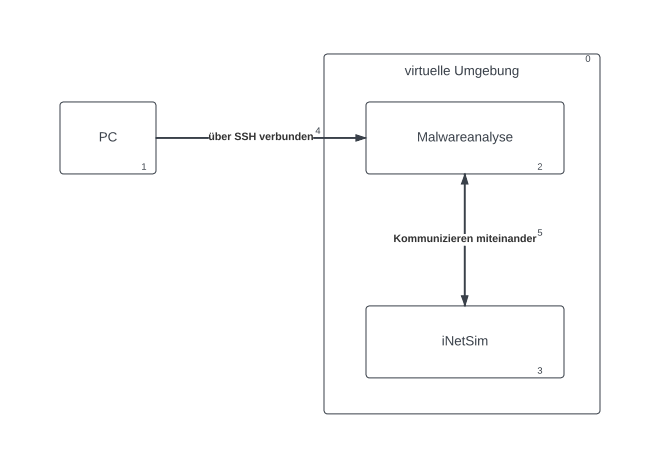
\includegraphics[scale=0.7]{LaTeX/graphic/virtuelleUmgebung.png}
    \caption{Aufbau der Cloud-Umgebung}
\end{figure}
\newline
In Abbildung zwei ist dieser Aufbau bildlich dargestellt. Auf der rechten Seite befindet sich die virtuelle Umgebung (mit null gekennzeichnet). Auf ihr laufen die beiden virtuellen Server. Einer der Server ist für die Malware-Analyse zuständig (mit zwei gekennzeichnet). Hier sind die Tools vorzufinden und die Malware wird hier eingeschleust. Außerdem gibt es den zweiten virtuellen Server, welcher ein Netzwerk simuliert (mit drei gekennzeichnet). Dafür wird das Programm \dq iNetSim \dq{} verwendet. Dieses simuliert gängige Internetdienste und ist dafür gemacht bei der Malware-Analyse eingesetzt zu werden.
\newline
Diese beiden Server können über jeden Port miteinander kommunizieren, haben aber keine Verbindung nach außen, sondern bleiben in der geschlossenen Umgebung. Die Kommunikation der beiden Server ist in der Abbildung mit fünf gekennzeichnet. Die einzige weitere Verbindung die in diesem System hergestellt wird ist die Verbindung vom PC des Benutzers auf den Malware-Analyseserver über SSH (mit vier gekennzeichnet). Somit wird gewährleistet, dass man als Analyst der Malware das System steuern und beobachten kann. 
\newline
Anhand des Aufbaus der Umgebung ist auch zu erkennen wie abgekapselt das System ist. Es bestehen keine Verbindungen nach außen, sondern nur untereinander, bzw von außen nach innen. Das ist auch wichtig um das Ausdringen der Malware zu verhindern. Diese Regeln für die Kommunikation sind in den Firewallregeln festgehalten. 
\subsection{Terraform}
\subsubsection{Verbindung mit dem Cloud-Provider}
Um Terraform als Provisioning-Tool für Cloud-Umgebungen zu verwenden, muss eine Verbindung zwischen der Terraform-Umgebung und dem Provider vorhanden sein. Diese Verbindung wird über ein API-Token geschaffen. Ein API-Token ist
\subsubsection{Konfiguration der Server}
In Terraform können Server erstellt und entsprechend konfiguriert werden. Wie das gemacht wird, wird hier einmal aufgegriffen. 
\newline
In HCL werden Blocks für die Erstellung von vielen Komponenten verwendet, darunter auch für die Servererstellung. 
\tt  
\begin{lstlisting}[caption = Konfiguration Malware-Server, language=python, numbers=left, numberstyle=\tiny]
# Create a server
resource "hcloud_server" "malware" {
  name        = "malware"
  image       = "ubuntu-22.04"
  server_type = "cx11"
  firewall_ids = [hcloud_firewall.saferfw.id]
  ssh_keys = [hcloud_ssh_key.default.id]
  user_data = file("user_data.yml")

public_net {
    ipv4_enabled = true
    ipv4 = hcloud_primary_ip.primary_ip_Malware.id
    ipv6_enabled = false
  }
}
\end{lstlisting}
\rm
Der abgebildete Code ist die Konfiguration für einen Server in der \dq Hetzner-Cloud\dq. Das ist bereits in Zeile zwei hinter \dq resource \dq{} zu erkennen. Der hier erstellte Server trägt den Namen \dq malware \dq{} und hat als Betriebssystem \it Ubuntu \rm (Vgl. Zeile vier). Der Server-Typ (Zeile 5) legt fest, welche Cloud-Lösung des Providers verwendet werden soll. In der \dq Hetzner-Cloud \dq{} ist \dq cx11\dq{} die günstigste Version. Diese ist für die grundlegende Malware-Analyse dennoch ausreichend. Falls die Analyse durch stärkere Systemkomponenten beschleunigt werden soll, kann hier der Typ geändert werden. 
\newline
Im Anschluss daran wird dem Server eine Firewall zugewiesen. Welche Einstellungen diese hat wird im nächsten Unterpunkt genauer betrachtet. Daraufhin bekommt der Server die Info woher der SSH-Key genommen wird (Zeile sieben). In Zeile zehn werden die öffentlichen Netzwerkeinstellungen vorgenommen. Dazu wird festgelegt, welche \dq Internet-Protokoll-Version \dq{} vorhanden ist. In diesem Fall ist \dq IPv4 \dq{} erlaubt und \dq IPv6 \dq{} nicht. Die \dq IPv4 \dq-Adresse wird dem Server fest zugewiesen. Das ist für die spätere Kommunikation mit dem anderen Server wichtig.
\newline
\newline
\tt  
\begin{lstlisting}[caption = Konfiguration iNetSim-Server, language=python, numbers=left, numberstyle=\tiny]
#Create second Server
resource "hcloud_server" "iNetSim" {
  name        = "iNetSim"
  image       = "ubuntu-22.04"
  server_type = "cx11"
  firewall_ids = [hcloud_firewall.iNetSimFW.id]
  ssh_keys = [hcloud_ssh_key.default.id]
  
  public_net {
    ipv4_enabled = true
    ipv4 = hcloud_primary_ip.primary_ip_iNetSim.id
    ipv6_enabled = false
  }
}
\end{lstlisting}
\rm
Die Konfiguration des zweiten Servers ist, wie hier zu sehen, sehr ähnlich zu der des ersten Servers. Der Unterschied hier ist nur die zugewiesene Firewall (Zeile sechs) und die IP-Adresse (Zeile elf). 
\subsubsection{Konfiguration der Firewall}
Die Erstellung einer sicheren und durchdachten Firewall ist bei der Arbeit mit Malware sehr wichtig, um Schäden am eigenen oder fremden Systemen zu vermeiden. 
\newline
\newline
\tt
\begin{lstlisting}[caption = Konfiguration der Firewall für den Analyseserver, language=python, numbers=left, numberstyle=\tiny]
#Create a firwall
resource "hcloud_firewall" "saferfw" {
  name = "saferfw"
  rule {
    direction = "in"
    protocol  = "tcp"
    port      = "22"
    source_ips = [
      "0.0.0.0/0",
      "::/0"
    ]
  }

  rule {
    direction = "out"
    protocol  = "udp"
    port = "1-65535"
    source_ips = [
      hcloud_primaryip.primary_ip_iNetSim.id
    ]
  }

  rule {
    direction = "out"
    protocol = "tcp"
    port = "1-65535"
    source_ips = [
      hcloud_primaryip.primary_ip_iNetSim.id
    ]
  }
}
\end{lstlisting}
\rm
Dieser Code stellt die Definition der Firewall für den Malware-Analyseserver dar. Der Name dieser Firewall ist \dq saferfw \dq{} und sie besteht aus drei Regeln. Die erste Regel (Zeile vier bis elf) legt die Kommunikation über den SSH-Port fest. Diese ist nur nach innen zugelassen. Wer diese Verbindung zum Server herstellt ist egal, solange der SSH-Key stimmt. 
\subsection{Tools}
Für eine ausführliche Analyse der vorliegenden Malware werden Tools benötigt. Ziel ist hierbei, dass die Tools die statische und dynamische Analyse abdecken. So kann die Malware in der Umgebung vollumfänglich untersucht werden. Für die Analyse von Malware in Linux-Systemen gibt es bereits viele Möglichkeiten. Betriebssysteme wie \dq Kali-Linux\footnote{} \dq{} oder auch \dq Remnux\footnote{} \dq{} sind Linux-Varianten, die speziell für die Analyse von schädlichen Programmen ausgelegt sind. Hier sind bereits viele Tools vorinstalliert. Obwohl die Arbeit mit den eben genannten Betriebssystemen die Auswahl der Tools vereinfachen würde, werden diese hier nicht verwendet. Viele Cloud-Provider bieten für virtuelle Server diese Betriebssysteme nämlich nicht an. Stattdessen wird auf den hier erstellten virtuellen Servern Ubuntu als Linuxdistribution verwendet. Dieses ist bei vielen Cloud-Anbietern verfügbar und unterstützt somit das Ziel der Flexibilität der Umgebung. 
\newline
Als erstes geht es um die Tools für die statische Analyse. \dq TrID \dq{} ist zum Identifizieren von Dateien sehr nützlich. Die Daten, mit denen festgestellt wird, um was für eine Art von Datei es sich handelt werden aus einer Datenbank bezogen, die mit dem Programm verknüpft ist. Diese wächst immer weiter, sodass hier nicht mit veralteten Datenbanken gearbeitet wird. Das sichert die Verlässlichkeit der Daten. Zum Zeitpunkt der Recherche wird dieses Tool immer noch regelmäßig aktualisiert, was die Aktualität der Datenbanken unterstreicht.\footcite{TrID} 
\newline 
Für die erweiterte statische Analyse werden Disassembler und Decompiler verwendet. Diese helfen dabei, die Funktionsweise der schädlichen Datei zu verstehen. Dafür wird die Maschinensprache die der Computer interpretieren kann in eine für Menschen lesbare Sprache umgewandelt. Das Programm \dq Ghidra \dq{} ist für diesen Zweck sehr geeignet. Ghidra wurde ursprünglich für den Geheimdienst der USA entwickelt und ist nun als Open-Source-Software erhältlich. Es interpretiert die Maschinensprache und erzeugt aus einem ausführbaren Programm einen Code um, der für Menschen verständlich ist. So kann die Vorgehensweise des zu untersuchenden Programms analysiert und verstanden werden.\footcite{}
\newline
Als Debugger wird in dieser Cloud-Umgebung \dq GNU Debugger (GDB) \dq{} benutzt. Dies ist ein weiteres Tool, welches in einer Linuxumgebung für die Analyse von Schadcode verwendet werden kann. Es wird für die dynamische Analyse verwendet. \dq GDB \dq{} wird dafür verwendet, Programme zu starten und festzustellen, was das verhalten des gestarteten Programms beeinflussen kann. Außerdem können Bedingungen für den Start und Stop des Programmes festgelegt werden. Zudem wird dokumentiert was das Programm gemacht hat, sobald es gestoppt wurde.\footcite{}
\newline


\subsection{Wie die Malware auf die virtuelle Umgebung gelangt}
Die virtuelle Umgebung soll zur gezielten Analyse von Malware-Samples verwendet werden. Anders als bei \it Honeypods \rm, die Malware \dq anlocken \dq{}, gelangt die Schadsoftware also nicht zufällig auf das System, sondern muss gezielt heruntergeladen werden. 
\newline
Zuerst stellt sich die Frage, woher man die Malware bekommt. Wird sie einem zugeschickt mit der Aufgabe sie zu untersuchen ist sie meist bereits verpackt und über einen Download-Link abrufbar. Wird die Malware auf einem System gefunden und man möchte sie untersuchen, sollte man die zum Schadcode gehörenden Dateien verpacken. Dazu eignet sich das Dateiformat \dq Tar \dq{} sehr gut. Bei Dateien mit der Endung \dq .tar \dq{} werden alle zu verpackenden Dateien in einer Datei zusammengeführt. Der Inhalt dieser Datei ist erst nach dem entpacken wieder sichtbar. 
\newline
Wenn das Malware-Sample verpackt ist, bietet es sich an die Malware über einen Download-Link bereitzustellen. In dieser Arbeit ist diese Plattform \dq Seafile \dq. Auf der Cloud-Umgebung ist die Malware anschließend über das Kommando: \newline \tt wget [DOWNLOAD-LINK]\rm \newline herunterladbar. Dies kann nur erfolgen, wenn die Firewall ausgeschaltet ist, da in dieser die Kommunikation in das Internet verboten ist. Ist der verpackte Schadcode auf der Cloud-Umgebung, muss die Firewall wieder aktiviert werden. Anschließend kann die Malware für die Analyse entpackt werden. Dies geschieht unter Linux mit dem Kommando: \newline \tt tar -xvzf [NAMEDERDATEI]. tar. gz \rm \newline
Ab diesem Zeitpunkt ist die Malware auf der Analyseumgebung angekommen und ist bereit für die Analyse.
\newpage
\end{otherlanguage}
\begin{otherlanguage}{ngerman}
\subsection{Tools}
Für eine ausführliche Analyse der vorliegenden Malware werden Tools benötigt. Ziel ist hierbei, dass die Tools die statische und dynamische Analyse abdecken. So kann die Malware in der Umgebung vollumfänglich untersucht werden. Für die Analyse von Malware in Linux-Systemen gibt es bereits viele Möglichkeiten. Betriebssysteme wie \dq Kali-Linux\footnote{} \dq{} oder auch \dq Remnux\footnote{} \dq{} sind Linux-Varianten, die speziell für die Analyse von schädlichen Programmen ausgelegt sind. Hier sind bereits viele Tools vorinstalliert. Obwohl die Arbeit mit den eben genannten Betriebssystemen die Auswahl der Tools vereinfachen würde, werden diese hier nicht verwendet. Viele Cloud-Provider bieten für virtuelle Server diese Betriebssysteme nämlich nicht an. Stattdessen wird auf den hier erstellten virtuellen Servern Ubuntu als Linuxdistribution verwendet. Dieses ist bei vielen Cloud-Anbietern verfügbar und unterstützt somit das Ziel der Flexibilität der Umgebung. 
\newline
Als erstes geht es um die Tools für die statische Analyse. \dq TrID \dq{} ist zum Identifizieren von Dateien sehr nützlich. Die Daten, mit denen festgestellt wird, um was für eine Art von Datei es sich handelt werden aus einer Datenbank bezogen, die mit dem Programm verknüpft ist. Diese wächst immer weiter, sodass hier nicht mit veralteten Datenbanken gearbeitet wird. Das sichert die Verlässlichkeit der Daten. Zum Zeitpunkt der Recherche wird dieses Tool immer noch regelmäßig aktualisiert, was die Aktualität der Datenbanken unterstreicht.\footcite{TrID} 
\newline 
Für die erweiterte statische Analyse werden Disassembler und Decompiler verwendet. Diese helfen dabei, die Funktionsweise der schädlichen Datei zu verstehen. Dafür wird die Maschinensprache die der Computer interpretieren kann in eine für Menschen lesbare Sprache umgewandelt. Das Programm \dq Ghidra \dq{} ist für diesen Zweck sehr geeignet. Ghidra wurde ursprünglich für den Geheimdienst der USA entwickelt und ist nun als Open-Source-Software erhältlich. Es interpretiert die Maschinensprache und erzeugt aus einem ausführbaren Programm einen Code um, der für Menschen verständlich ist. So kann die Vorgehensweise des zu untersuchenden Programms analysiert und verstanden werden.\footcite{}
\newline
Als Debugger wird in dieser Cloud-Umgebung \dq GNU Debugger (GDB) \dq{} benutzt. Dies ist ein weiteres Tool, welches in einer Linuxumgebung für die Analyse von Schadcode verwendet werden kann. Es wird für die dynamische Analyse verwendet. \dq GDB \dq{} wird dafür verwendet, Programme zu starten und festzustellen, was das verhalten des gestarteten Programms beeinflussen kann. Außerdem können Bedingungen für den Start und Stop des Programmes festgelegt werden. Zudem wird dokumentiert was das Programm gemacht hat, sobald es gestoppt wurde.\footcite{}
\newline


\subsection{Wie die Malware auf die virtuelle Umgebung gelangt}
Die virtuelle Umgebung soll zur gezielten Analyse von Malware-Samples verwendet werden. Anders als bei \it Honeypods \rm, die Malware \dq anlocken \dq{}, gelangt die Schadsoftware also nicht zufällig auf das System, sondern muss gezielt heruntergeladen werden. 
\newline
Zuerst stellt sich die Frage, woher man die Malware bekommt. Wird sie einem zugeschickt mit der Aufgabe sie zu untersuchen ist sie meist bereits verpackt und über einen Download-Link abrufbar. Wird die Malware auf einem System gefunden und man möchte sie untersuchen, sollte man die zum Schadcode gehörenden Dateien verpacken. Dazu eignet sich das Dateiformat \dq Tar \dq{} sehr gut. Bei Dateien mit der Endung \dq .tar \dq{} werden alle zu verpackenden Dateien in einer Datei zusammengeführt. Der Inhalt dieser Datei ist erst nach dem entpacken wieder sichtbar. 
\newline
Wenn das Malware-Sample verpackt ist, bietet es sich an die Malware über einen Download-Link bereitzustellen. In dieser Arbeit ist diese Plattform \dq Seafile \dq. Auf der Cloud-Umgebung ist die Malware anschließend über das Kommando: \newline \tt wget [DOWNLOAD-LINK]\rm \newline herunterladbar. Dies kann nur erfolgen, wenn die Firewall ausgeschaltet ist, da in dieser die Kommunikation in das Internet verboten ist. Ist der verpackte Schadcode auf der Cloud-Umgebung, muss die Firewall wieder aktiviert werden. Anschließend kann die Malware für die Analyse entpackt werden. Dies geschieht unter Linux mit dem Kommando: \newline \tt tar -xvzf [NAMEDERDATEI]. tar. gz \rm \newline
Ab diesem Zeitpunkt ist die Malware auf der Analyseumgebung angekommen und ist bereit für die Analyse.
\newpage
\end{otherlanguage}

\lhead{Ergebnisse}
%Ergebnisse
\section{Ergebnisse}
Als Endprodukt dieser Arbeit sind zwei virtuelle Server auf einer virtuellen Umgebung entstanden, die zur Analyse von Malware genutzt werden kann. Was jedoch auch zu beachten ist ist, dass dies nicht das einzige Ergebnis ist. Dahinter steckt nämlich ein Skript für Terraform, welches individuell an die Gegebenheiten und den jeweiligen Provider angepasst werden kann. Zudem können Tools in diesem Skript, je nach Bedarf, variabel ausgetauscht werden. Ansonsten sind die Tools so ausgewählt, dass sie die bestmöglichen Bedingungen für die Analyse von Malware bieten.
\newpage


\lhead{Diskussion}
%Diskussion
\begin{otherlanguage}{ngerman}
\section{Diskussion}
\subsection{Analyse der Ergebnisse}
\subsection{Bewertung der Ergebnisse}
\subsection{Ausblick}
Eine angemessene Benutzerfreundlichkeit ist ein wichtiger Punkt dieser Arbeit. Eine virtuelle Umgebung ist ohne Benutzerhandbuch teilweise schwer zu durchblicken und daher nicht wirklich benutzerfreundlich. Um dem Benutzer dabei etwas an die Hand zu geben ist die Erstellung eines \it Wikis\rm. Dieses soll als Benutzerhandbuch dienen und die wichtigsten Bereiche und Hinweise zur Erstellung und Verwendung der virtuellen Umgebung abdecken. Zu jeder Funktionalität sollen hier Begründungen und Hinweise zu finden sein. Außerdem werden an manchen Punkten Alternativen oder Verbesserungsmöglichkeiten aufgezeigt werden. 
\end{otherlanguage}
\lhead{Fazit}
%Fazit
\section{Fazit}
\subsection{Zusammenfassung der Ergebnisse}
Zusammenfassend kann festgehalten werden, dass das Ziel der Arbeit erreicht wurde. Es wurde eine flexible Cloud-Umgebung erstellt, die die entsprechenden Malware-Analyse-Tools zur Verfügung stellt. Festzuhalten ist dennoch, dass diese Umgebung noch nicht perfekt ist und immer noch Verbesserungsbedarf besteht. Dennoch ist sie für die Analyse von Malware geeignet und wird, um die vollständige Funtkionsfähigkeit zu gewährleisten, stetig überarbeitet und verbessert. Mithilfe dieser Umgebung ist die Grundlage dafür geschaffen worden, die Funktionsweise von Malware besser zu verstehen. Sie ist außerdem die Verbindung von zwei Themenbereichen der Informationstechnik. Hier werden Infrastructure-as-Code-Tools, speziell Terraform, in Verbindung mit der Erstellung einer Malware-Analyse-Umgebung gebracht. Diese zwei Themenfelder sind in gemeinsamer Verbindung wenig erforscht, jedoch gibt es hier ein hohes Potential. 


\lhead{Literatur- und Quellenverzeichnis}
\section{Literatur- und Quellenverzeichnis}
%%%%%%%%%%%%%%%%%%%%%%%%%%%%
%% Literaturverzeichnis wird 
%% automatisch eingefügt
%%%%%%%%%%%%%%%%%%%%%%%%%%%%

\printbibliography
\addcontentsline{toc}{section}{Literatur- und Quellenverzeichnis}
aufteilen in internetquellen
publications
books

\newpage
\lhead{Anhang}
\section{Anhang}
\appendix
\section{Anhang A} 





%%%%%%%%%%%%%%%%%%%%%%%%%%%%
%% Eidesstattliche Erklärung
%%%%%%%%%%%%%%%%%%%%%%%%%%%%
\clearpage
\newpage
\begin{otherlanguage}{ngerman}
\thispagestyle{empty}
\section*{Eidesstattliche Erklärung}
\thispagestyle{empty}
Hiermit versichere ich, die vorliegende Arbeit selbstständig verfasst und keine anderen als die angegebenen Quellen und Hilfsmittel benutzt sowie die Zitate deutlich kenntlich gemacht zu haben.
\newline
Ich erkläre weiterhin, dass die vorliegende Arbeit in gleicher oder ähnlicher Form noch nicht im Rahmen eines
anderen Prüfungsverfahrens eingereicht wurde.
\vspace{4\baselineskip}\\
Berlin, den \today \hfill Patrick Lucas Büdke 
\vspace{4\baselineskip}\\
\end{otherlanguage}

\end{document}
